\documentclass[12pt]{article}
\usepackage[utf8]{inputenc}
\usepackage{color,lineno,setspace,graphicx,multirow,kpfonts}
\usepackage[top=2.4cm,left=2.4cm,top=2.4cm,bottom=2.4cm,includefoot]{geometry}
\usepackage[style=bes]{biblatex}
\bibliography{./library, EKLOF,CHEUNG,THUILLER,CANARD, POISOT, WILLIAMS, HAVENS, BAISER, PEREIRA, WHITEHEAD, STOUFFER, STOU2, ALLESINA, ALLOUCHE, ALBOUY, FROESE, JACKSON,STANKO}
%\bibliograph{library}

\begin{document}

\linenumbers 
\modulolinenumbers[1]

\textbf{Title:}   Inferring food web structure from predator-prey body size relationships\\

\textbf{Authors:}  Dominique Gravel$^{1,2,*}$, Timoth\'ee Poisot$^{1,2}$, Camille Albouy$^{3,4}$, Laure Velez$^{3}$, David Mouillot$^{3,5}$\\

1: Canada Research Chair on Terrestrial Ecosystems. D\'epartement de biologie, chimie et g\'eographique, Universit\'e du Qu\'ebec \`a Rimouski, 300 All\'ee des Ursulines, Qu\'ebec, Canada. G5L 3A1.\\

2: Qu\'ebec Centre for Biodiversity Sciences, Stewart Biological Sciences Building, 1205 Dr.~Penfield Avenue, Montr\'eal (QC), H3A 1B1, Canada

3: UMR CNRS-UM2-IRD-IFREMER 5119 ECOSYM, Universit\'e Montpellier 2, CC 093, 34095 Montpellier Cedex5, France.\\

4: Laboratoire Ecosystèmes Marins Exploit\'es UMR 212, IRD, IFREMER, UMII, UMI, avenue Jean Monnet BP171, 34203 Sete Cedex, France.\\

5: ARC Centre of Excellence for Coral Reef Studies, James Cook University, Townsville, Qld 4811, Australia\\

* Corresponding author. {\tt dominique\_gravel@uqar.ca}. Tel: 1-418-723-1986 \#1752. Fax: 1-418-724-1849.\\

\textbf{Keywords:} Metaweb, Body size, Niche model, Food web\\

\textbf{Words in the abstract:}      179

\textbf{Words in the main text:}     2819

\textbf{Words in the legends:}       423

\textbf{References:}                   45

\textbf{Figures:}                       6

\textbf{Table:}                         0

\newpage
\doublespacing

\section*{Abstract}

Current global changes make it important to be able to predict which
interactions will occur in emerging ecosystems. Most of the current methods to
infer the existence of interactions between two species require a good knowledge
of their behaviour or a direct observation of interactions. In this paper, we
overcome these limitations by developing a method, inspired from the niche model
of food web structure, using the statistical relationship between predator and
prey body size to infer the matrix of potential interactions among a pool of
species. The novelty of our approach is to infer, for any species of a given
species pool, the three species specific parameters of the niche model. The
method applies to both local and metaweb scales. It allows one to evaluate the
feeding interactions of a new species entering the community. We find that this
method gives robust predictions of the structure of food webs, and that its
efficiency is increased when the strength of the body- size relationship between
predators and preys increases. We finally illustrate the potential of the method
to infer the metaweb structure of pelagic fishes of the Meditarrannean sea under
different global change scenarios.

\newpage

%------------------------------------------------------------
\section{Introduction}
One of the current challenges in ecology is to predict the emergence and
re-assembly of communities following species responses to global changes.
Understanding this is made all the more important as these novel ecosystems will
be more common with increasing human pressure. We know that species invasions,
biomass harvesting, ranges shifts, disturbances and changes in land use are
important drivers of biodiversity turnover. How they affect species composition
is now well described \parencite{Pereira2010}, but forecasting their impact on
community structure and functioning requires \emph{a priori} knowledge of
potential interactions among species. Predicting interactions among species that
never co-occurred proves challenging, as traditional empirical methods of food
web sampling such as stomacal content analysis cannot be applied. While for
competitive communities this task could be achieved using predictive modeling
based on functional traits \parencite{McGill2006, Albouy2010} or phylogeny
\parencite{Cavender-Bares2009, Mouquet2012} , it is much more difficult to
forecast trophic interactions in a food web \parencite{Ings2009,
Tylianakis2008,Montoya2010}.

Inferring potential interactions among species of an arbitrary defined pool is a
major step to predict the structure of emergent communities and their
functioning. We call these potential interactions among a given set of species, wether
at the local or regional scales, the \emph{metaweb} \parencite{Dunne2006}. A
metaweb takes the form of an adjacency matrix $\mathbf{MW}$, of size $s\times s$
for a pool of $s$ species, and in which $\mathbf{MW_{ij}} = 1$ if species $i$
can consume species $j$, and $0$ otherwise. This matrix aggregates the trophic
interactions among all species from the pool that are susceptible to both
co-occur and interact at the regional scale \parencite{Dunne2006}. With a
metaweb in hands, one could analyze the impacts of global changes, such as range
shifts or species invasions, on the potential community structure, by extracting
the relevant species and examining the properties of the community they define.
While this concept is progressively finding its way through theoretical spatial
food web ecology \parencite{Lafferty2010, Pillai2009, Gravel2011a, Gravel2011b},
it is still limited by data availability and predictive accuracy. Published
metaweb data rely on literature surveys \parencite{Havens1992, Piechnik2008,
Baiser2012}, or a compilation of several local food webs \parencite{Stanko2002,
Poisot2012a}, making them resolved only for species that co-occurred a large
enough number of times.

Development of predictive models of trophic interactions could greatly improve
our understanding of large scale food web structure and our capacity to
anticipate major changes in ecosystem functionning. Theory should provide some
guidance about the general rules underpinning interactions among a set of
species and thus help us to infer the metaweb. The actual food web theory is
largely derived from the niche model \parencite{Williams2000}. This model simply
and intuitively poses that each species in a food web has a niche position
$n_i$, a feeding niche optimum $c_i$ and a range $r_i$ of suitable preys around
that optimum (Fig. 1). These simples rules are sufficient to generate realistic
food web structures that fit most of published food webs \parencite{Dunne2006}.
The niche model was a substantial improvement of the previous cascade model
(Cohen1990) and subsequent models (e.g. the nested hierachy model
\parencite{Cattin2004}, the minimum potential model \parencite{Allesina2008},
the probabilistic niche model \parencite{Williams2010} are somehow derived from
these rules \parencite{Stouffer2005}. Although it is based on different
assumptions, the adaptive foraging theory of food web structure
\parencite{Petchey2008b} provides comparable predictions
\parencite{Williams2010}. One major recent breakthrough in food web theory have
been the attempts to parameterize the niche model and other food web models from
field data and to compare their fit through likelihood methods
\parencite{Allesina2008, Williams2010, Williams2011}. These methods provide, for
each species of the food web, the optimal parameters to fit the empirical web
structures, given the hypothesized underlying rules of the niche model.

Despite their theoretical interest, these methods however come with several
drawbacks when comes the time to perform biodiversity scenarios. Firstly, they
are difficult to apply at large scale because of the technical and logistical
requirements of metaweb data collection. Secondly, once the model is
parameterized, it could only be used to infer feeding interactions between
species with already documented interactions (i.e. it is impossible to infer
potential interactions among species that do never co-occurred). Finally, the
model optimization is a serious challenge for large datasets with a large number
of parameters to evaluate and rough likelihood surfaces. There is consequently
an urgent need for a method that could rapidly and easily provide an estimate of
potential interactions in a metaweb based on incomplete data.

In this paper, we present a method designed to infer the potential interactions
between all pairs of species of a species pool based on observations of body
size of predators and their prey. The method applies to both the local and the
metaweb scales. We do so by a parameterization of the niche model, based on the
well-documented allometric scaling relationship between predator and prey
\parencite{Cohen2003, Brose2006, Riede2010}. We first develop the method and
apply it to food webs from various environments. We find the method accurately
predicts the interactions (and lack thereof), and that the accuracy increases
with the strength of the predator-prey body size relationship. We then analyze
the sensitivity of the method to incomplete data (missing links) and find that
it is robust to sampling effort. We finally illustrate the potential of the
method to infer the metaweb structure of pelagic fishes of the Meditarrannean
sea and the consequences of alteration of body size distribution by global
changes or anthropic forcings. The method is best suited for strongly
size-structured food webs and will likely not hold for other types of
non-body-size structured interactions. We therefore conclude on the future
issues to generalize this approach to other types of trait matching models.

%------------------------------------------------------------
\section{Model description}

The method aims to infer the potential interactions among a pool of species from
a subset of observations of predator-prey interactions. The method follows the
following steps, with details provided below:
\begin{description}
\item[Step 1:] Log transformation of the body size data;
\item[Step 2:] Statistical analysis of the predator-prey body size relationship;
\item[Step 3:] Inferrence of the niche model parameters for all species from the species pool;
\item[Step 4:] Interpretation of the parameters and computation of the metaweb.
\end{description}
We also provide an example of R code (R Core Development Team) and data in the Supplementary Material, detailling the step by step procedure and the format of the input data. 

%------------------------------------------------------------
\subsection{Inferring parameters from the niche model and building the metaweb}

The niche model predicts the food web structure from a set of three
species-specific parameters \parencite{Williams2000}: the niche position $n_i$,
the feeding niche optimum $c_i$ (called the centroid), and the feeding range
$r_i$. A species $i$ will predate all species $j$ whose niche position $n_j$
lies within the interval $[c_i-r_i/2,c_i+r_i/2]$ (Fig. 1). We evaluate all of
these parameters from the predator-prey body size relationship, enabling us to
parameterize the metaweb from \emph{observed} interactions only. The
parameterization is robust to the sampling effort, as it is much easier to
document interactions than their absence \parencite{Martinez1999}. Our approach
is however mostly limited to predatory interactions since the body size
relationship between herbivores and primary producers is not as general
\parencite{Riede2010}, and obviously do not hold for parasitic, mutualistic, or
competitive networks.

Assuming that body size is the main niche axis structuring trophic interactions,
the parameter $n_i$ corresponds simply to the log of body size (in mass or
length) of species $i$. Though only the relative position of all species along
the body size gradient needs to be respected, it is possible to standardize log
body size values between 0 (minimum size in the regional species pool) and 1
(maximal size). We then consider a linear relationship between the decimal
logarithm of body size and the centroid of the niche (the dark line at Fig. 1).
This relationship is obtained by fitting the linear model $c =
\mathrm{log}_{10}(M_{prey})=\alpha_0 +
\alpha_1\times\mathrm{log}_{10}(M_{pred})$ to the data, where $M_{prey}$ and
$M_{pred}$ are the prey and predator body size respectively. The lower and upper
boundaries of the feeding range are easily obtained by fitting the 5\% and 95\%
quantile regressions between $\mathrm{log}_{10}(M_{prey})$ and
$\mathrm{log}_{10}(M_{pred})$ (the dotted lines at Fig. 1, see the example at
Fig. 2). We note them as $r_{low,i}$ and $r_{high,j}$ respectively, and the
corresponding parameters of the linear quantile regresions are
$\beta_{0,low/high}$ and $\beta_{1,low/high}$. In sum, the parameter $n_i$ for
any species of the metaweb is given by the standardized value of the log body
size $M_i$, $c_i$ is estimated from the linear regression between predator and
prey log body size and $r_i$ from the quantile regressions. Type I regressions
were used because there is no equivalence of type II models for quantile
regressions.

The next step of the methodology is to reconstruct the metaweb. Once these
parameters are calculated from a subsample of species from the regional pool,
the coefficients of the different linear models are used to infer the niche
parameters of each species of the species pool. Again, the niche parameter for
any species $i$, $n_i$, is given by the log of body size. The centroid of the
niche is obtained by the relationship $c_i = \alpha_0 +
\alpha_1\times\mathrm{n_i}$, the lower boundary of the niche is $r_{low,i} =
\beta_{0,low} + \alpha_{1,low}\times\mathrm{n_i}$ and the upper boundary
$r_{high,i} = \beta_{0,high} + \alpha_{1,high}\times\mathrm{n_i}$. A feeding
link from species $j$ to species $i$ occurs if $n_j > r_{low,i} \& n_j <
r_{high,i}$. We provide an example at Fig. 2.

%------------------------------------------------------------
\section{Method accuracy}
\subsection{Predictive performance}
We illustrate the method with the food web datasets of Brose et al.
\parencite{Brose2005}. The meta-analysis of Brose \parencite{Brose2006} was
conducted on this dataset to test the generality of the predator-prey body size
relationship across different systems (terrestrial, aquatic and marine). The
relationship was found to be very strong across all systems despite exhibiting
variability from one to another. Each web has between 26 and 380 species and 18
and 1466 feeding links. Several of these webs are repetitions over time at a
single location, in which cases we pooled the data for each of the 15 different
locations to calculate the predator-prey body size relationship. We removed 4
datasets that had a non-significant predator-prey relationship and were thus
useless with our approach. The links are not systematically sampled, meaning
that any absence of a link between two species for a given dataset could either
be a real absence or due to insufficient sampling or lack of information. While
the predator-prey body size relationship is very strong over all datasets
(Brose2006), there is quite substantial variation among them, enabling us to
assess the sensitivity of the method to the strength of this relationship.

We assessed the performance of our method using the True Skill Statistic
($TSS$). The $TSS$ is based on the partition of events (the prediction of a
trophic interaction) between four components: the component $a$ reports the
number of links that are both predicted and observed, $b$ reports predicted
links with no corresponding observation, $c$ reports the number of observed
links that are predicted absent, and $d$ reports the number of predicted and
observed absences of links. The TSS is then calculated as $TSS
=(ad-bc)/\left[(a+c)(b+d)\right]$. The $TSS$ quantifies the proportion of
prediction success relative to false predictions and returns values ranging
between 1 (perfect predictions) and -1 (inverted forecast)
\parencite{Allouche2006}.

We calculated the $TSS$ for each of the 11 different webs and related it to the
strength of the predator-prey body size relationship, measured by the $R^2$ of
the linear model. We find that the $TSS$ is positive for all webs, ranging from
0.13 to 0.76 (Fig. 3A). We find a positive relationship between the $R^2$ of the
linear model and the $TSS$ ($R^2=0.50$, $p=0.016$). When we decompose the
different components of predictions and observations, we find that the fraction
of prediction match is high, with an average of
$(\overline{a}+\overline{d})/{S^2}=0.58$, Fig. 3B). The fraction of wrong
predictions is lower, at $\overline{b+c}/S^2=0.40$, and decreases with the $R^2$
of the predator-prey body size relationship.

The parameterized niche model tends to overestimate the number of links in a web
(see the example at Fig. 2). This result is significant but not surprising,
given that these datasets do not necessarily contain all links, as they were not
designed with this purpose, and thus some of the links might have been missed.
This interpretation is also reminiscent of previous debates on the difficulty to
sample all links in a web \parencite{Martinez1999}. It is also well known that
the niche model predicts a continuous diet along the niche axis (the webs are
said to be interval \parencite{Cohen1990, Stouffer2006}), while real food webs
do not have this characteristic. We thus might over predict link density within
the niche of a given species. Previous studies \parencite{Allesina2008} and the
Application 1 however show this problem is easily circumvented when a second
niche axis, \emph{e.g.} an environmental niche, comes into play. A recent study
on dimensionality of networks shown that most webs have between 3 and 6
dimensions \parencite{Eklof2013}, meaning that adding a few more niche axes can
greatly improve the accuracy of predictions.

%------------------------------------------------------------
\subsection{Sensitivity to sampling effort}
We subsequently explored the impact of sampling effort on the accuracy of the
model predictions. We assumed a random subsampling of all the interactions
occurring in the food web. To do so, we selected a species rich food web ($S =
67$) from the Brose et al. dataset, with 601 observed feeding links and a good
$TSS$ (0.51). We randomly removed from 0 to $90\%$ of the observed links to do
the evaluation of the parameters of the linear regressions (i.e. e decrease the
quantity of information used to calibrate the model). We then after compared the
empirical web (with all species) to the inferred web with these parameters (all
species also). The comparison was done again with the TSS. We performed 100
randomizations per number of removed links. This numerical simulation reproduces
incomplete sampling in the process of building the food web. We find that the
$TSS$ remains constant up until $80\%$ of the observed links are removed (Fig.
3). At this level, the $TSS$ starts to decline drastically and its variance
increases.

This result shows that our method of parameterization of the niche model is
robust with regard to sampling effort. Note however that a biased sampling with
respect to body size (e.g. sampling of the largest species) might be more likely
to reduce the fit of the predator-prey body size relationship. The aggregation
intro trophic species that do have the same body size and the same diet should
not impact the prediction since it will not affect parameter evaluation. It will
however reduce the fit of the predator-prey body size relationship and therfore
the accuracy of the method if the species do have different body sizes. The same
artifact will be observed if there is strong intraspecific variation in body
size (see the Discussion).

%------------------------------------------------------------
\section{Application: Mediterranean food web structure under fishing pressure}
\subsection{Dataset}
We now present an application of the method to infer the metaweb of interactions
among fishes of the Mediterranean sea. The Mediterranean is known as a hotspot
of fish diversity that is severely threatened by climate change and overfishing
\parencite{Mouillot2011}.There are 557 fish species in the regional pool, with a
maximum body size ranging from 2.3 cm to 1100 cm \parencite{Whithead1986,
Louisy2005, Froese2011}. Chondrichthyans, mammals and turtles were under
represented in the two trophic networks and were removed from the analyses. We
parameterized the niche model with a subset of species, from two different
highly resolved food webs from the Catalan area \parencite{Coll2006} (82
species) and Corsica \parencite{Albouy2010} (58 species).

\subsection{Inferring the metaweb for Mediterrannean fishes}
We estimated parameters $n$, $c$ and $r$ for each of the 557 species and
inferred the potential interactions among all of them (the example in the
Supplementariy code is based on this dataset). The metaweb has a total of 126
501 links, for a connectance of 0.41 (Fig. 5A). The metaweb is also highly
nested (specialist species feed on a subset of prey of the most generalist
species. Fig. 5A). We also considered a second niche axis related to species
spatial distribution. Most fish species have restricted geographic range within
the Mediterranean sea because of specific response to temperature and other
environmental variables \parencite{Albouy2012}. We therefore removed from the
metaweb all links between species having no range overlap. Data on the extent of
occurrence of fish species were compiled from a published atlas of fishes of the
northern Atlantic and the Mediterranean \parencite{Whitehead1986}. This atlas is
based on regional data sets and expert knowledge and was edited between 1984 and
1986. It currently provides the only available basin-wide information on the
extent of occurrence of all Mediterranean Sea fish species. The above mentioned
atlas do not account for the bathymetric distribution of Mediterranean fish
species, yet bathymetry is considered as one of the main factors accounting for
marine fish distributions \parencite{Louisy2005}. We therefore refined the
extent of occurrence maps by clipping off areas with depths that fall outside
the minimum or maximum known for the species. Species' bathymetric ranges were
obtained from FishBase \parencite{Froese2010, Louisy2005}. The resulting metaweb
has a total of 95 989 links, for a connectance of $C = 0.31$. Connectance
decreases because links are removed by incomptabilities in bathymetry but the
total number of species stays constant. This metaweb is clearly less interval
(Fig. 5B). Contiguous gaps in the diet are likely to emerge from modularity in
the co-occurrence matrix \parencite{Araujo2011}. Future studies should explore
how co-occurrence is constraining the topological structure of metawebs.

%------------------------------------------------------------
\subsection{Impact of global changes}
Our method to parameterize the niche model has a unique feature relative to the
original niche model \parencite{Williams2000}: the network properties of the
original model, such as the number of links, food chain length and degree
distribution (the number of in and out feeding links per species), are
controlled by the input parameters (species richness and connectance), wherea
all properties of our parameterized niche model are emergent features of the
predator-prey body size relationship and the frequency distribution of body
size. The connectance in the niche model is fixed by the user; in our case it
strongly depends on the scaling of the feeding range with body size and the
frequency of larger body species.

This feature is particularly important to understand global change impacts on
community structure. For instance, a common prediction of the impact of
fisheries on the body size distribution is the reduction in the average and
variance of body size \parencite{Jackson2001}. Similarly, global warming is also
expected to alter fish body size distribution towards smaller species
\parencite{Cheung2012}. We explored by simulations the impact of these changes
on the degree distribution of the Mediterranean metaweb. Results are illustrated
at Fig. 6. The shape of the cumulative degree distribution provides a visual
assessment of the distribution of diet specificity in a network. The curves
becomes steeper and the fall moves to the left with increasing specialization
(indicative of a larger proportion of species with a low degree). Even if the
simulated scenarios are crude representations of the predicted alterations of
community structure, they both show that fisheries impacts on body size will
substantially alter the network properties. The results at Fig. 6 show that
reduction in the average body size will decrease the average number of preys per
predator (there is an initial sharper decline of the cumulative distribution),
but that super generalist species will also appear (because of the shift of the
tail toward the right). The removal of the 40\% largest species reduces much
more the average generality which is expected as larger species are predators
with a large feeding niche in the niche model. The two scenarios consequently
increases substantially the relative abundance of species with a smaller degree,
even for the average size reduction scenario where the total number of species
is held constant. The change in the degree distribution is likely to reduce
substantially the expected persistence and stability of these communities
\parencite{Gravel2011a, Gravel2011b}.

%------------------------------------------------------------
\section{Discussion}

In this paper, we presented a method to infer potential interactions among an
arbitrary pool of species. The data required to perform this methodology are
simple to obtain, as the body size of a large number of species are available
from reference databases, or easy to measure. Because we rely on a robust
allometric relationship, applying this method requires neither complex
statistical techniques, nor an exhaustive knowledge of the realized interactions
within the metaweb of interest. In addition to the opportunity to simulate
biodiversity scenarios, our method can also help generating baseline
expectations about the food web structure for environments which are notoriously
difficult to sample, such as soils, deep-sea environments, or fossil records.
However, because this allometric relationship is characteristic of predatory
interactions, our method will likely not hold for other types of non-body-size
structured interactions such as herbivory and parasitism.

It appears at Fig. 2 that the feeding range increases with the body size of the
predator. This result was quite general across datasets with a good fit of the
predator-prey body size relationship, although with considerable variation in
the slope of the relationship. It offers the possibility to compare empirical
based estimates of the parameters to the original niche model of
\textcite{Williams2000}. For this specific dataset that the model for the
centroid is $c_i = -1.34 + 0.66n_i$ and the average range
($\overline{r}_i=(r_{high,i} - r_{low,i})/2$) is $\overline{r}_i = 0.63 +
0.78n_i$. The original niche models assumed that $r_i$ scales linearly with
connectance $C$ and the niche position, such that $r_i = 2Cn_i$. Even though the
parameterization suggests a linear increase of generality with body size, the
final number of preys in the diet for a given size will depend on the frequency
distribution of body size. A large predator for instance could have a large
feeding range, but only few species to find on and effectively appears as a
specialist. This relationship will have to be investigated further, among
several food webs (e.g. \textcite{Digel2011}), because the scaling of generality
with trophic rank has several consequences on persistence
\parencite{Gravel2011b} and food web dynamics \parencite{Brose2006,Berlow2009}.

Ontogenic shifts in diet are common in many size-structured populations and
could be accounted for in two ways with this methodology. First, they will enter
the model parameterization by simply including a link from species A (the
largest) to species B (the smallest), and the opposite. This would yield in a
data point for species B figuring above the 1:1 relationship. Such a data point
will obviously influence the model calibration and enlarge the regime of all
species. It is not obvious however that ontogenic shifts will be found in the
metaweb as it would require an upper limit of the range above the 1:1
relationship. The alternative approach would be to distinguish "sub-species" by
size categories in the model calibration and then in the reconstruction of the
metaweb. This approach would force ontogenic shifts and perhaps more precisely
represent the interaction matrix where the within-population size structure is
important.

The method should be completed with other sources of informations to better
predict gaps in the interaction matrix. The original niche model was definitely
inspired by the predator-prey body size relationship, but was intented to be
more general and eventually deal with several niche axes
\parencite{Williams2000}. \textcite{Allesina2008} indeed found that adding a
second axis, creating gaps into the first axis interaction matrix, increases the
fit of the model to empirical data. It also makes the network less interval (a
continuous succession of species diets along the niche axis), a structural issue
of the niche model that was reported by \textcite{Cattin2004} and
\textcite{Bersier2006}. There are numerous sources of information that could be
used to improve the model, such as co-occurrence and functional traits.

Our application with the Mediterannean pelagic fish food web provides an example
of how straightforward it is to add additional information so as to improve the
parameterization. A similar approach could also build on the comptability of
other traits such as phenology, location in the water column or hunting modes.
While the approach we describe here is based on very simple statistics, the next
methodological efforts will also have to take into account more various and
heterogeneous sources of data such as phylogeny \parencite{Eklof2012} and expert
knowledge. Bayesian inference appears a good candidate to achieve goal. It
offers the possibility to constrain the prior distribution of the likelihood of
any pairwise interaction, based on trait matching, using alternative source of
data. The method we employed here was based on the match between predator and
prey traits. This method could be generalized by looking at the match between
all potential traits. \textcite{Eklof2013} indeed found that the match between
only three traits is enough to encompass a vast majority of interactions. But
when such data is not always available, then it might be possible to use
phylogeny as a proxy for a high dimensional trait species, provided that traits
are conserved along the phylogeny \parencite{Mouquet2012}. A bayesian addition
to the model would be to weight the likelihood that species $j$ is a predator of
species $i$, considering that the closest relative of this predator is also a
predator of $i$. It could account for part of the unexplained variation we found
in our analysis, for instance by constraining the range of the diet for some
large predators or by creating holes within the feeding range
\parencite{Rall2011}.

Adding this method to the ecologist's toolbox is a timely issue because there is
an urgent need to include interactions into future biodiversity scenarios
\parencite{Thuiller2013}. There has been impressive progress in biogeography
over the last fifteen years to predict the impact of global changes on range
shifts, extinction risks, and the future distribution of biodiversity, but we
now face the realization that emerging ecosystems are unlikely to be a spatial
displacement of the ones we currently know. This method will help assessing
global change impacts of community structure, moving the field of biogeography
closer to ecosystem functioning.

\section{Acknowledgements}
We thank I. Gounand for preparing the food web data. We also thank N. Martinez,
U. Brose and two anonymous reviewers for their constructive comments and
stimulating discussion. DG received financial support from NSERC and Canada
Research Chair program. TP is funded by a MELS-FQRNT post-doctoral fellowship.
\newpage

\printbibliography
\newpage

\section*{Figure legends}

\subsection*{Figure 1} 
Schematic representation of the niche model and its
application to the predator-prey body size relationship. Three consumer species
are represented. The white triangles correspond to the niche position of
predators (their position on the X axis is transposed along the Y axis). For
most cases, prey size is smaller that the predator size and thus fall under the
1:1 relationship. In some occasions, however, the feeding range can overlay the
1:1 relationship, for instance in presence of ontogenic shifts in diet. For a
given predator, we consider that the niche centroid ($c_i$) is the average prey
size, given by the linear relationship between predator and prey size (black
line). The boundaries of the feeding range ($r_i$) are given by the 5\% and 95\%
quantile regression lines (dotted lines). A predator feeds on all prey species
which their niche lies between these boundaries. In this specific example, the
largest predator feeds on the two smaller species (the white triangles depicting
the niche lies between range boundaries) and the intermediate size predator
feeds on the smallest species.

\subsection*{Figure 2} 
Example of predator-prey body size relationship and
predictions from the parameterized niche model. Open dots represent observed
links while black dots are predicted interactions based on the parameterization
of the niche model. The bullseye symbols thus correspond to a match between
predicted occurrence of a link and the real data (the "a" classification in the
calculation of the TSS, see main text), a black dot a predicted link with not
observation ("b") and an open circle a non-predicted and observed link ("c").
Data from a creek bed located in Australia \parencite{Brose2005}.

\subsection*{Figure 3} 
Performance of the parameterized niche model to predict
food web structure for the 11 food webs. A) Relationship between the TSS and the
$R^2$ of the predator-prey body size relationship. B) Partitionning of the
different components of the TSS.

\subsection*{Figure 4} 
Effect of the sampling effort on the accuracy of the
parameterized niche model to predict food web structure. The simulation was
conducted with the same data as Fig. 2.

\subsection*{Figure 5} 
Illustration of the metaweb of the Mediterannean pelagic
fishes (interactions in black). Panel A) represents the full metaweb and B) the
same metaweb for which links between species not co-occuring together were
removed (their range overlap for less than $0.1\%$ of the Mediterannean sea).

\subsection*{Figure 6} 
Impacts of altering the body size distribution of
Meditarrennean fishes on the degree distribution of the metaweb. The black line
corresponds to the original metaweb degree distribution. For the first scenario,
we simulated a $40\%$ reduction in average body size and recalculated the
metaweb properties, keeping the predator-prey body size relationship constant
(dotted line). For the second scenario we eliminated the top $40\%$ largest
species and recalculated the metaweb properties (dashed line).

\newpage
\section*{Figures}

\subsection*{Figure 1}

\begin{figure}[ht!]
	\centering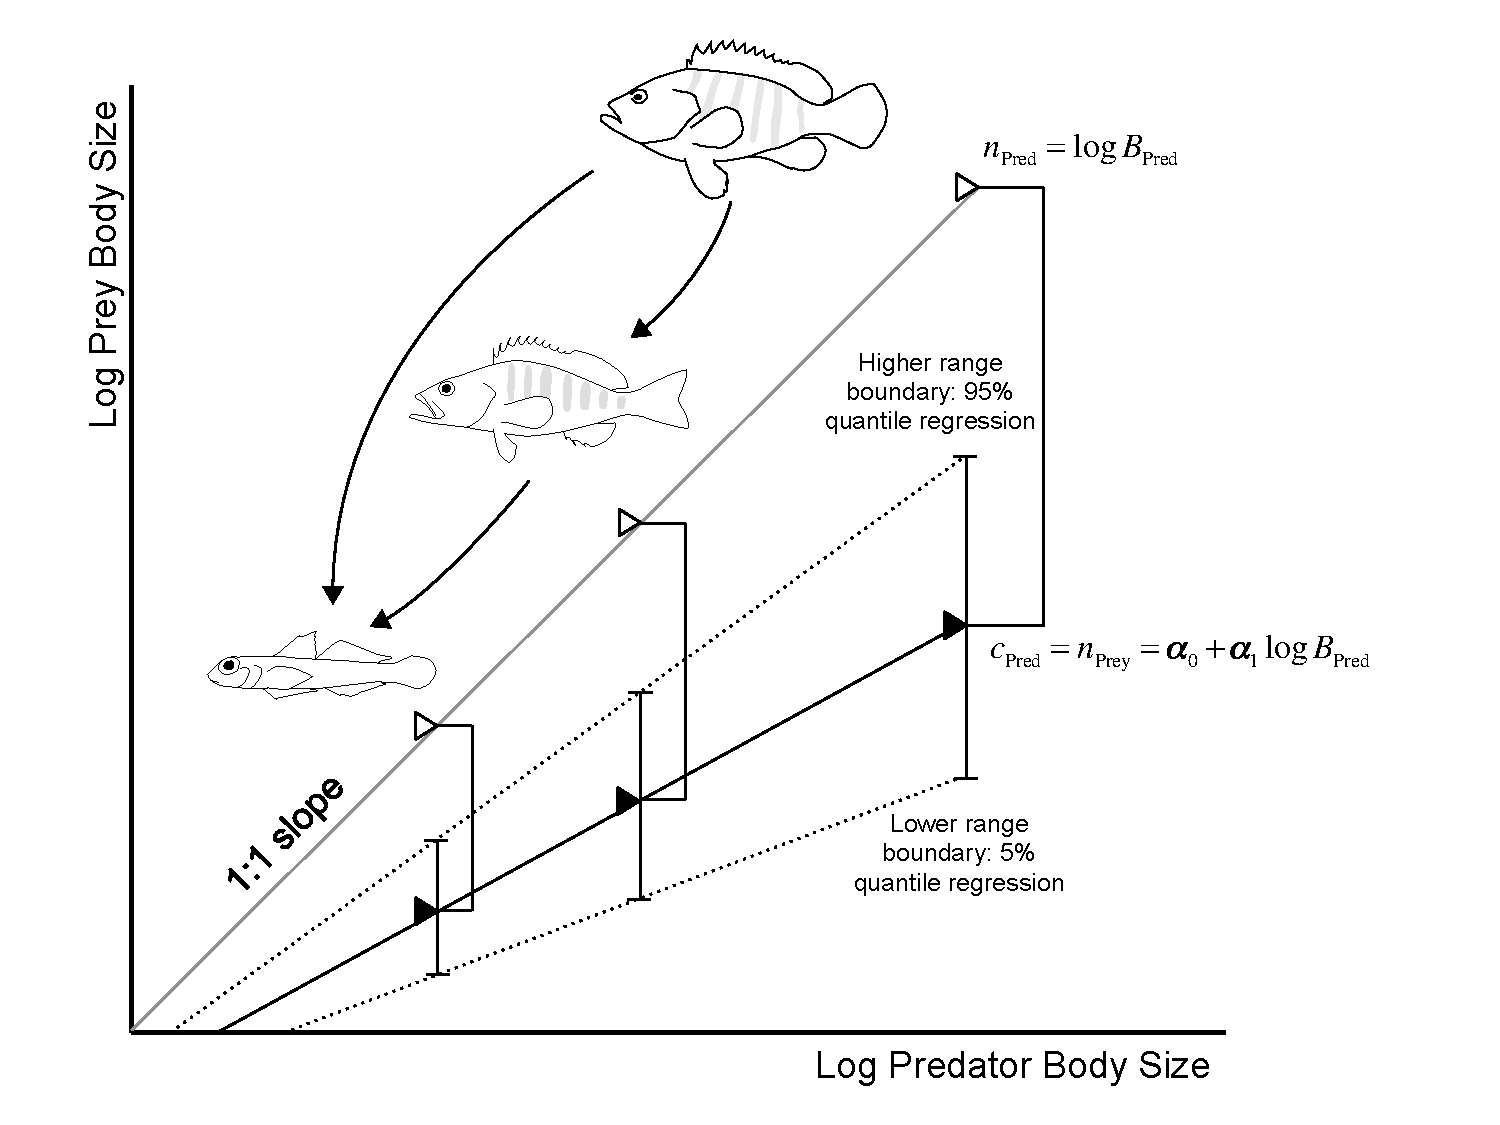
\includegraphics[width=0.85\textwidth]{Schema_niche_allometric.pdf}
\end{figure}

\newpage
\subsection*{Figure 2}

\begin{figure}[ht!]
	\centering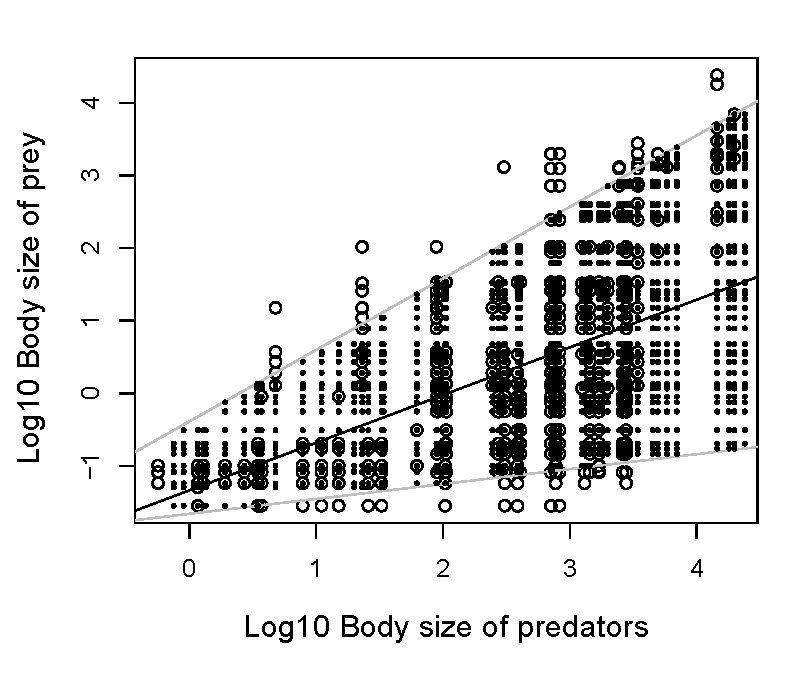
\includegraphics[width=0.85\textwidth]{Example.pdf}
\end{figure}

\newpage
\subsection*{Figure 3}

\begin{figure}[ht!]
	\centering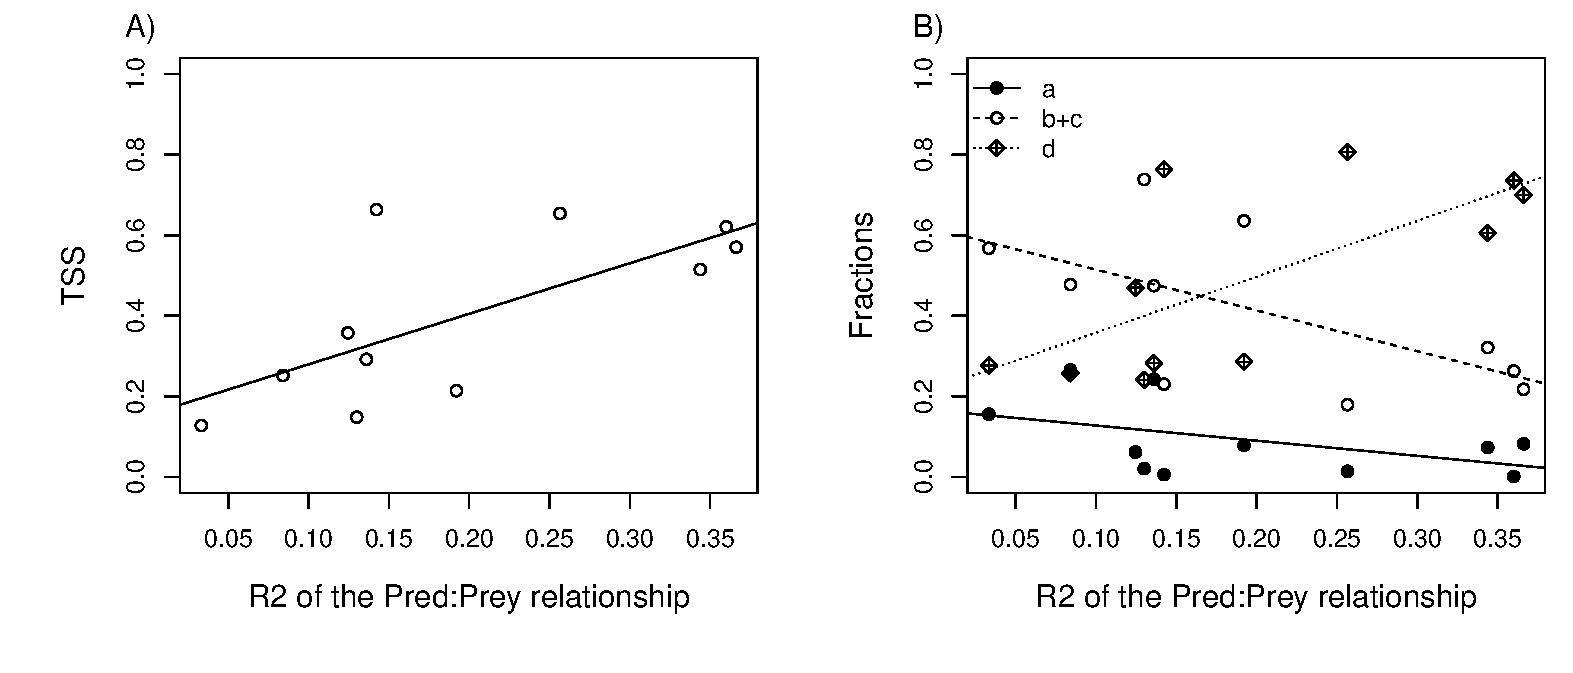
\includegraphics[width=1\textwidth]{TSS_perweb.pdf}
\end{figure}

\newpage
\subsection*{Figure 4}

\begin{figure}[ht!]
	\centering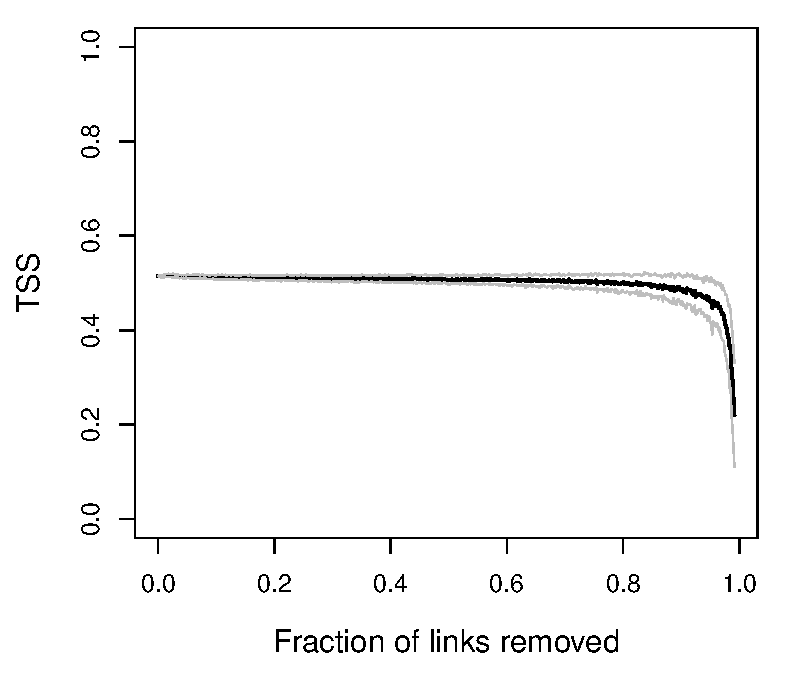
\includegraphics[width=0.85\textwidth]{TSS_sampling.pdf}
\end{figure}

\newpage
\subsection*{Figure 5}

\begin{figure}[ht!]
	\centering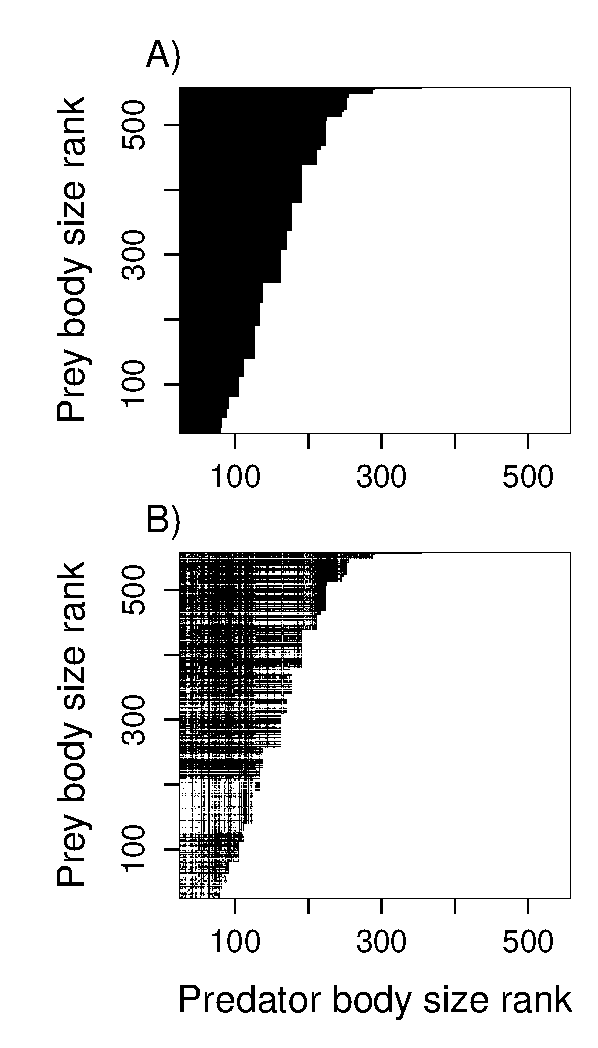
\includegraphics[width=0.6\textwidth]{Example_MED.pdf}
\end{figure}

\newpage
\subsection*{Figure 6}

\begin{figure}[ht!]
	\centering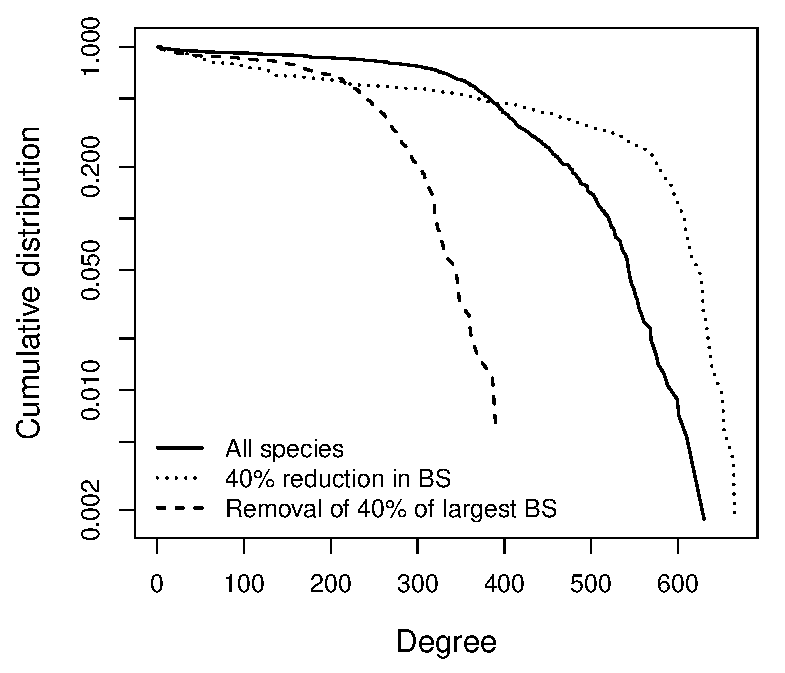
\includegraphics[width=0.85\textwidth]{Degree.pdf}
\end{figure}

\end{document}

